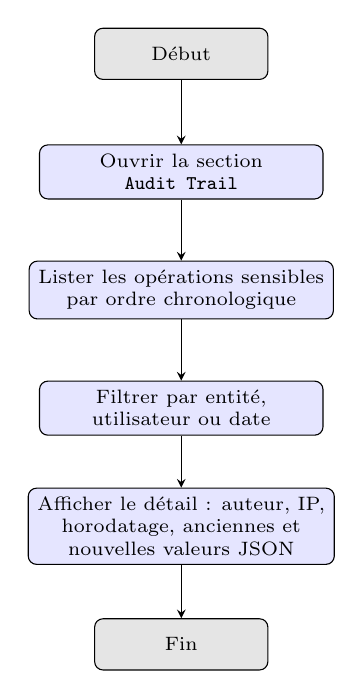
\begin{tikzpicture}[font=\scriptsize, >=stealth,
  startstop/.style={rectangle, rounded corners=3pt, fill=gray!20, draw=black, minimum width=2.2cm, minimum height=0.65cm, align=center},
  action/.style={rectangle, rounded corners=3pt, fill=blue!10, draw=black, minimum width=3.6cm, minimum height=0.65cm, align=center},
  decision/.style={diamond, draw=black, fill=orange!10, aspect=2, text width=2.6cm, align=center, inner sep=1pt},
  edgelabel/.style={font=\tiny, fill=white, inner sep=1pt}]

\node[startstop] (debut) at (0, 0) {D\'ebut};
\node[action] (ouvrir) at (0, -1.5) {Ouvrir la section\\\texttt{Audit Trail}};
\node[action] (lister) at (0, -3.0) {Lister les op\'erations sensibles\\par ordre chronologique};
\node[action] (filtrer) at (0, -4.5) {Filtrer par entit\'e,\\utilisateur ou date};
\node[action] (detail) at (0, -6.0) {Afficher le d\'etail : auteur, IP,\\horodatage, anciennes et\\nouvelles valeurs JSON};
\node[startstop] (fin) at (0, -7.5) {Fin};

\draw[->] (debut) -- (ouvrir);
\draw[->] (ouvrir) -- (lister);
\draw[->] (lister) -- (filtrer);
\draw[->] (filtrer) -- (detail);
\draw[->] (detail) -- (fin);
\end{tikzpicture}